\documentclass[tikz,border=5pt]{standalone}
\usepackage[T1]{fontenc}
\usepackage{lmodern,amsmath,amssymb}
\usetikzlibrary{arrows.meta,calc,positioning,fit,backgrounds,shapes.geometric,matrix,decorations.pathreplacing,patterns}
\definecolor{ink}{gray}{0.08}
\definecolor{wash}{gray}{0.965}
\definecolor{soft}{gray}{0.45}
\tikzset{box/.style={draw=ink,line width=.65pt,fill=white,align=center,inner sep=4pt,outer sep=0pt,font=\small},flow/.style={draw=ink,line width=.65pt,-{Latex[length=1.8mm,width=1.3mm]},rounded corners=2pt},annotation/.style={font=\scriptsize,text=soft,align=center},groupbox/.style={draw=soft,dashed,line width=.45pt,fill=wash}}
\begin{document}
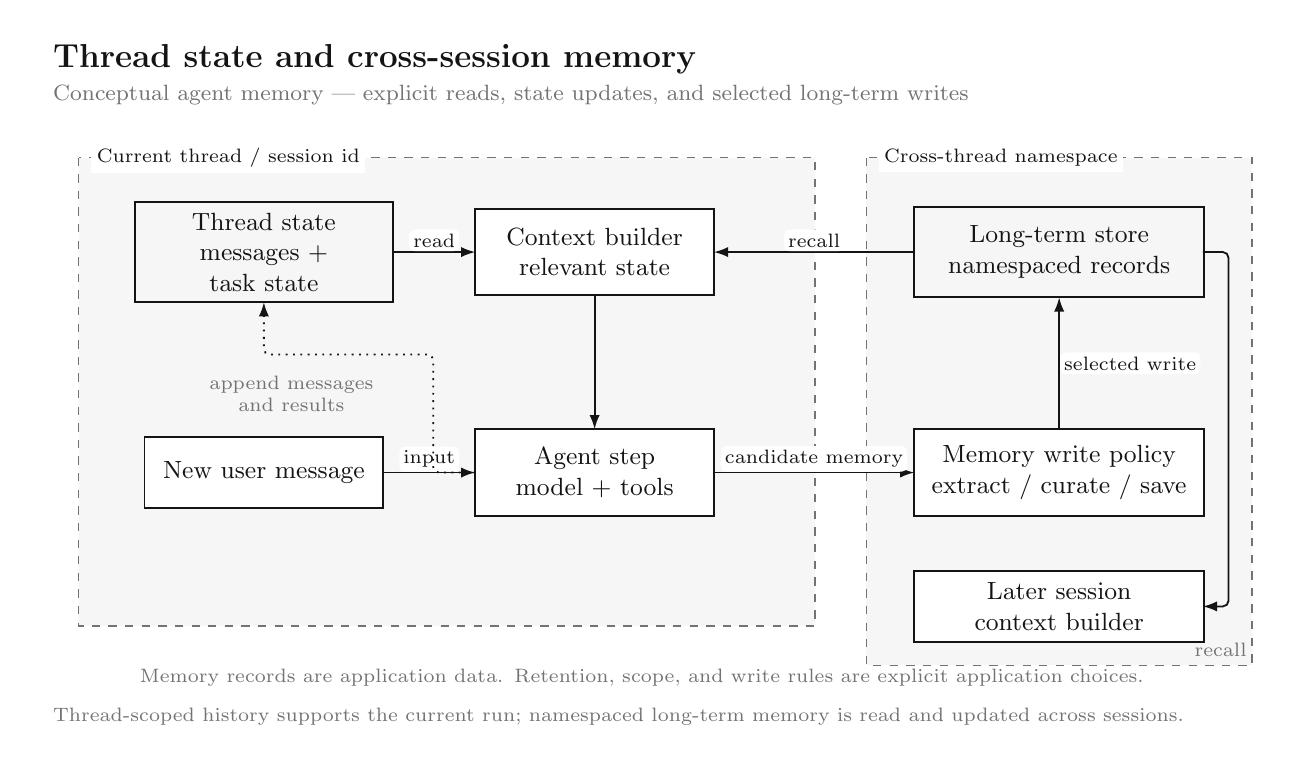
\begin{tikzpicture}[x=1cm,y=-1cm,font=\rmfamily,text=ink]

\path[use as bounding box] (0,0) rectangle (16,9);
\node[anchor=west,font=\large\bfseries] at (.2,.4) {Thread state and cross-session memory};
\node[anchor=west,font=\footnotesize,text=soft] at (.2,.85) {Conceptual agent memory | explicit reads, state updates, and selected long-term writes};
\begin{pgfonlayer}{background}
\draw[groupbox] (0.65,1.65) rectangle (10.0,7.6);
\node[anchor=west,font=\scriptsize,fill=white,inner sep=2pt] at (0.8,1.65) {Current thread / session id};
\draw[groupbox] (10.65,1.65) rectangle (15.55,8.1);
\node[anchor=west,font=\scriptsize,fill=white,inner sep=2pt] at (10.8,1.65) {Cross-thread namespace};
\end{pgfonlayer}
\node[box,fill=wash,minimum width=3.25cm,minimum height=1.15cm,text width=3.0cm] (history) at (3.0,2.85) {Thread state\\messages + task state};
\node[box,minimum width=3.0cm,minimum height=1.1cm,text width=2.75cm] (context) at (7.2,2.85) {Context builder\\relevant state};
\node[box,minimum width=3.0cm,minimum height=0.9cm,text width=2.75cm] (input) at (3.0,5.65) {New user message};
\node[box,minimum width=3.0cm,minimum height=1.1cm,text width=2.75cm] (agent) at (7.2,5.65) {Agent step\\model + tools};
\node[box,fill=wash,minimum width=3.65cm,minimum height=1.15cm,text width=3.4cm] (long) at (13.1,2.85) {Long-term store\\namespaced records};
\node[box,minimum width=3.65cm,minimum height=1.1cm,text width=3.4cm] (write) at (13.1,5.65) {Memory write policy\\extract / curate / save};
\node[box,minimum width=3.65cm,minimum height=0.9cm,text width=3.4cm] (next) at (13.1,7.35) {Later session\\context builder};
\begin{pgfonlayer}{background}
\draw[flow] (history.east) -- (context.west) node[midway,above,fill=white,inner sep=1.5pt,font=\scriptsize] {read};
\draw[flow] (context.south) -- (agent.north);
\draw[flow] (input.east) -- (agent.west) node[midway,above,fill=white,inner sep=1.5pt,font=\scriptsize] {input};
\draw[flow,dotted] (agent.west) -- (5.15,5.65) -- (5.15,4.15) -- (3,4.15) -- (history.south);
\draw[flow] (long.west) -- (context.east) node[midway,above,fill=white,inner sep=1.5pt,font=\scriptsize] {recall};
\draw[flow] (agent.east) -- (write.west) node[midway,above,fill=white,inner sep=1.5pt,font=\scriptsize] {candidate memory};
\draw[flow] (write.north) -- (long.south) node[midway,right,fill=white,inner sep=1.5pt,font=\scriptsize] {selected write};
\end{pgfonlayer}
\node[annotation,anchor=center,text width=3.0cm] at (3.35,4.65) {append messages\\and results};
\draw[flow] (14.925,2.85) -- (15.25,2.85) -- (15.25,7.35) -- (14.925,7.35);
\node[annotation,anchor=center,text width=1.1cm] at (15.15,7.9) {recall};
\node[annotation,anchor=center,text width=14.5cm] at (7.8,8.25) {Memory records are application data. Retention, scope, and write rules are explicit application choices.};
\node[anchor=west,align=left,font=\scriptsize,text=soft,text width=15.6cm] at (.2,8.75) {Thread-scoped history supports the current run; namespaced long-term memory is read and updated across sessions.};
\end{tikzpicture}
\end{document}
